\chapter{Design and materials}



\section{Basics on solar-charging systems and MPPT approaches }
A typical solar-charging system consists of solar arrays, MPPT controllers, power
electronic converters and loads. Efficiency increasing in each part caused improving
the solar-charging system. The single diode model of solar cell is illustrated in Fig 2.1. By putting the solar cells next to each other, the module will be obtained. A panel consists
of connecting several modules, and an array consists of connecting several panels.
The connections between these different modes can be done in series or in parallel.
For example, a solar panel is created by connecting a series or parallel of modules.
\begin{figure}[h]
	\centering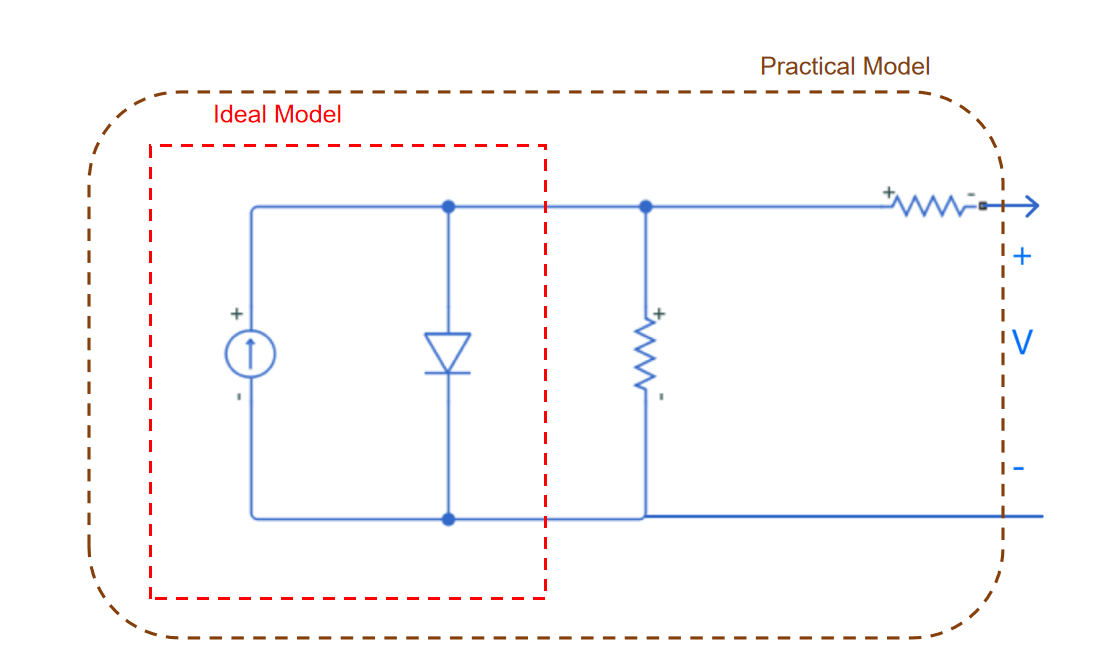
\includegraphics[height=3.5cm]{./images/single diode circuit}
	\caption{single diode circuit}
\end{figure}
\subsection{operation principle of a MPPT system}
Solar power-voltage characteristics' curve is presented in Fig. 1.
\begin{figure}[h]
	\centering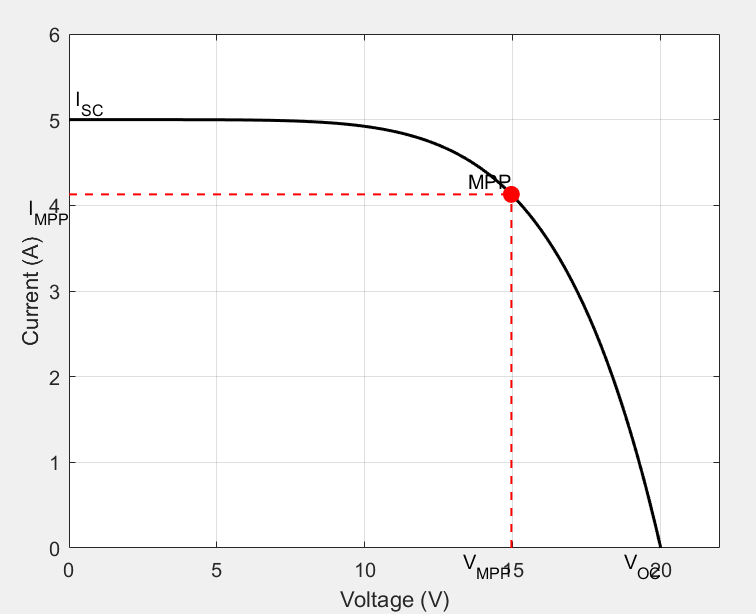
\includegraphics[height=4cm]{./images/current-voltage}
	\caption{current-voltage}
\end{figure}
The MPP is created near the top of the P-V curve, or the famous knee point of the P-V curve, where the generated PV power is maximized. As the MPP depends on solar radiation (S) and temperature (T), and these environmental conditions vary randomly, the MPP position is continuously changed. In order to ensure the operation point is always on the maximum power point, or near it, specific circuits, called MPP trackers, are employed. The DC-DC also applies the controller signal and brings the output to the desired level. Thus, by measuring different parameters (voltage, current or temperature), the maximum power point tracking algorithms calculate the optimal duty cycle (D) and deliver it to the converter to increase the power. Figure 2.3 shows the overview of PV system.
As it is known, the MPP system must operate continuously in real time because the parameters to which the system depends (temperature and radiation) change throughout the day. Changes in the amount of radiations and temperature during the day are  perfectly normal or there may be partial shading. As a result, duty cycle needs to be updated accurately and rapidly (as appropriate).

\begin{figure}[h]
	\centering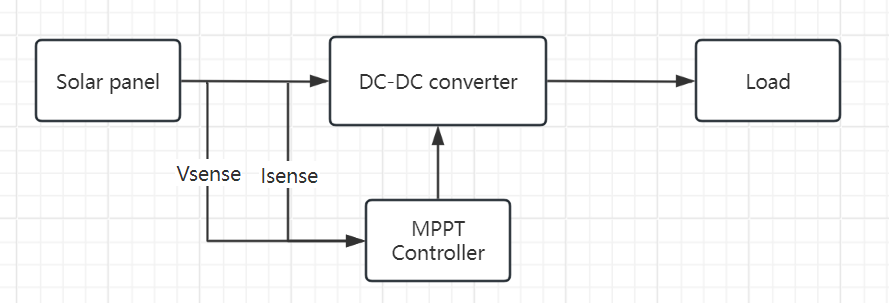
\includegraphics[height=3cm]{./images/Implementation of MPPT system}
	\caption{Implementation of MPPT system}
\end{figure}


\section{Materials}



Important: do not provide results in this section.

